\setlength{\footskip}{8mm}
\chapter{ Methodology } \label{methodology}
The chapter describes the methodology for the design and implementation of the system. 

\section{Camera Calibration}
Since I did not calibrate the camera I followed the 
following steps to get the intrinsic and extrinsic parameters of the camera.  

\begin{figure}
\centering
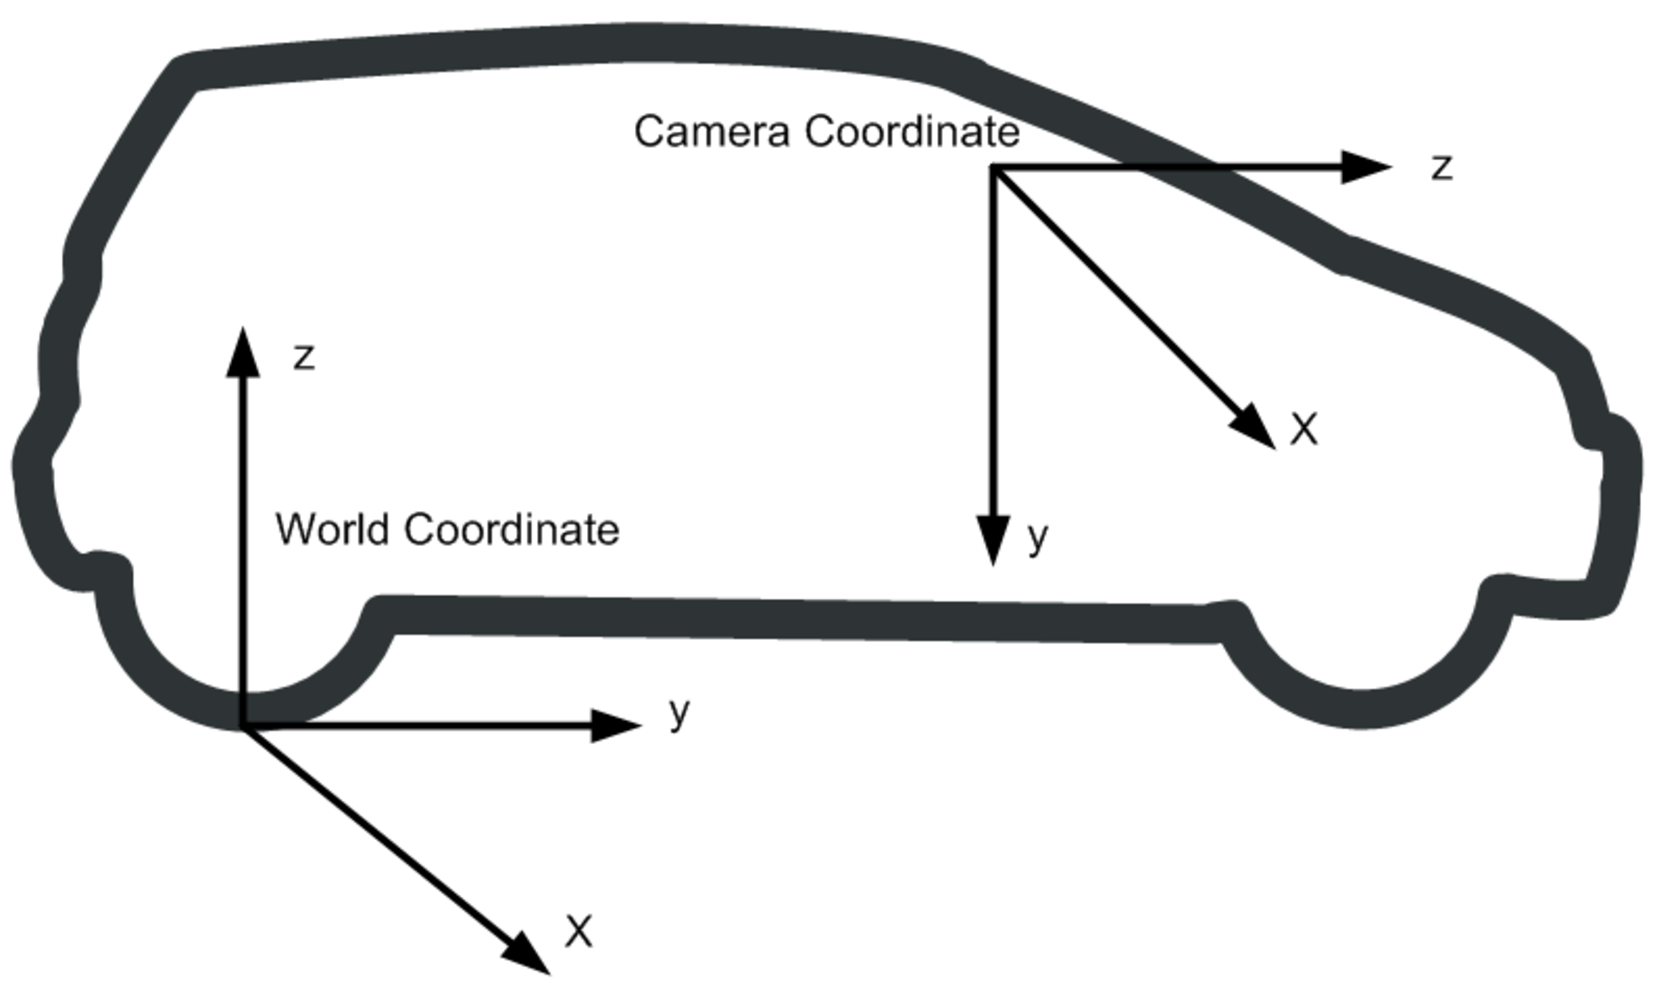
\includegraphics[width=110mm]{figures/camera-car-coordinate-system3.pdf}
\caption{The relationship between world and car coordinate system.}
\label{fig:camera_car_coordinate}
\end{figure}

\subsection{Intrinsic Parameters}
\begin{itemize}
  \item Focal Length: Every picture taken by a digital camera contains some meta 
data such as camera model, dimensions, color space, focal length, etc. The focal 
length obtained from the meta data is in millimeters where as the focal length 
that is needed in the camera matrix must be in pixels. Using the following 
equation\fullcite{FocalLength} I was able to convert the focal length from 
millimeters to pixels.  
\[ \text{focal length in pixels} =
     \text{image width in pixels} \times 
     \frac{\text{focal length in mm}} {\text{CCD width in in mm}} 
\]
  
The value of CCD can be obtained from the camera specifications. 
\item Principal Point: I assumed the principal point $(p_{x}, p_{y})$ to be at 
the center of the image. 
\item Skew: Skewing arise when the $x$ and $y$ axes of the pixel element are not 
perpendicular to each other. This is a very rare condition and it is safe to 
assume $s = 0$. 
\end{itemize}

\subsection{Extrinsic Parameters}
As described in Section \ref{sec:camera_calibration} the extrinsic parameters 
consists of the rotational matrix $\mat{R}$ and translation vector $\vec{t}$. 

Estimating the rotational matrix $\mat{R}$ without camera calibration is hard, since it depends on the yaw, pitch and roll of the camera. Thus, I conducted a simple experiment to estimate the rotational matrix. 

Assume three points $\vec{X_{1}}, \vec{X_{2}}, \vec{X_{3}}$ in the homogenous 
world coordinate system such that $\vec{X_{1}} = 
\begin{bmatrix}0&\beta&0&1\end{bmatrix}^{T}$, $\vec{X_{2}} = 
\begin{bmatrix}1&\beta&0&1\end{bmatrix}^{T}$, $\vec{X_{3}} = 
\begin{bmatrix}0&\beta&1&1\end{bmatrix}^{T}$ where $\beta$ is a large number so 
that the point $\vec{X_{1}}$ will be projected on the horizontal row of the 
image. Using Equation \ref{eq:camera_equation} and \ref{eq:camera_equation_2} 
the points $X_{1}, X_{2}, X_{3}$ are projected onto the image. Thus, 

\begin{center}
\begin{tabular}{c c c}
  $\vec{x_{1}} = \mat{K}[\mat{R}\mid\vec{t}]\vec{X_{1}}$, & 
  $\vec{x_{2}} = \mat{K}[\mat{R}\mid\vec{t}]\vec{X_{2}}$ &
  $\vec{x_{3}} = \mat{K}[\mat{R}\mid\vec{t}]\vec{X_{3}}$
\end{tabular}
\end{center}

From the above equation it can be seen that $\vec{x_{1}}, \vec{x_{2}}, \vec{x_{3}}$ depends on 
$\mat{R}$, which needs to be estimated. Since we know that $\vec{x_{1}}$ should be on 
the horizontal row and at the center of the lane and $\vec{x_{2}}, \vec{x_{3}}$ being 
slightly to the right and top of $\vec{x_{1}}$. $\mat{R}$ is adjusted until the condition is 
met. 

Figure \ref{fig:rotation_matrix}(a) shows the three points $\vec{x_{1}}$(red), 
$\vec{x_{2}}$(green), $\vec{x_{3}}$(blue) being off to the right. Figure 
\ref{fig:rotation_matrix}(b) shows the results of tuning the rotational matrix 
$\mat{R}$ so that the thee points are in the center of the lane.

\begin{figure}
 \centering
 \begin{tabular}{c c}
   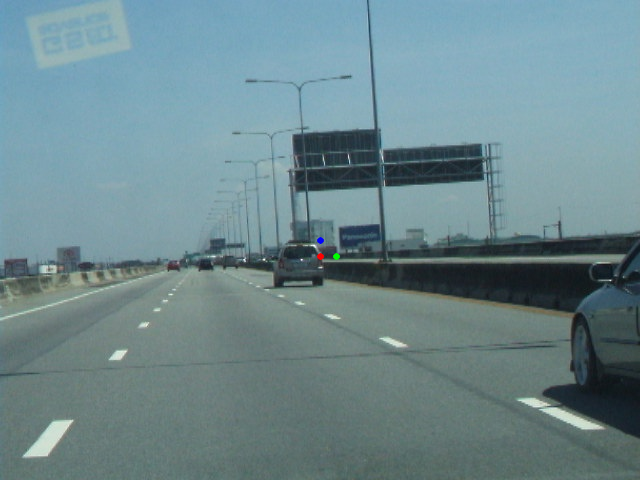
\includegraphics[width=80mm]{figures/rotation_after.png} &
   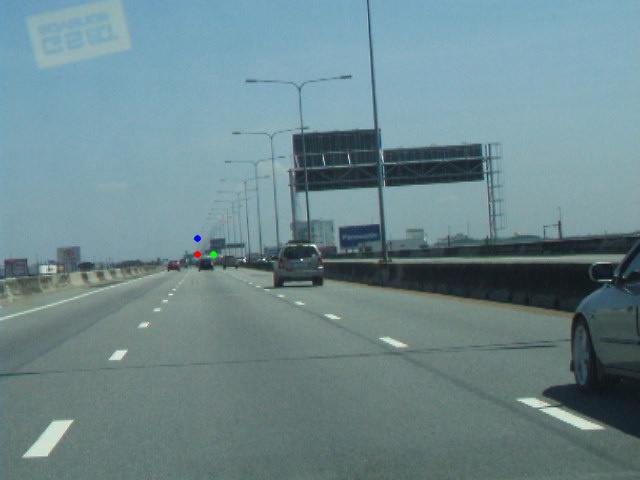
\includegraphics[width=80mm]{figures/rotation_before.png} \\
   (a) & (b) \\
 \end{tabular}
 \caption{Estimating the Rotation Matrix by using 3 points}
 \label{fig:rotation_matrix}
\end{figure}

The translation vector $\vec{t}$ is the distance from the world to camera 
coordinate system. This is the distance between the two wheels in the $y$ axis 
and the distance from the ground to the camera in the $z$ axis.

\section{Road Lane Extraction}
To detect the road lane marking I used the ``Road Paint Detection using Matched
Filters" algorithm \fullcite{huang2008rss}

\subsection{Calculating lane width in pixels}
The first step is to construct the matched filter. The matched filter varies 
depending on the lane width at each row of the image. Therefore in order to 
construct the matched filter the lane width at each row of the image must be 
calculated. Given that the camera matrix has already been determined as 
described in Section \ref{sec:camera_calibration}. A point in the image is 
related to a point in the real world by:
\begin{equation}\vec{x} \sim \mat{P}\vec{X} \end{equation} \label{eq:camera_eq}
As shown in Figure \ref{fig:camera_car_coordinate} the $z$ co-ordinate points 
upward to the sky therefore the $x,y$ plane is the ground plane. Assuming that 
the ground is flat $Z$ can be estimated to be $0$. 
\[
\begin{bmatrix}x\\y\\1\end{bmatrix}  \sim 
\mat{P} \begin{bmatrix}X\\Y\\0\\1\end{bmatrix}
\]
\begin{eqnarray*}
\begin{bmatrix}x\\y\\1\end{bmatrix} & = & 
\begin{bmatrix}
p_{11} & p_{12} & p_{13} & p_{14} \\
p_{21} & p_{22} & p_{23} & p_{24} \\
p_{31} & p_{32} & p_{33} & p_{34}
\end{bmatrix}
\begin{bmatrix}X\\Y\\0\\1\end{bmatrix}
\end{eqnarray*}
\begin{eqnarray*}
\begin{bmatrix}x\\y\\1\end{bmatrix} & = & 
\begin{bmatrix}
        Xp_{11} & Yp_{12} & \cancelto{0}{p_{13}} & p_{14} \\
        Xp_{21} & Yp_{22} & \cancelto{0}{p_{23}} & p_{24} \\
        Xp_{31} & Yp_{32} & \cancelto{0}{p_{33}} & p_{34}
\end{bmatrix} \\
\end{eqnarray*}
Since we are using homogenous coordinates therefore, 
\begin{eqnarray*}
y = \frac {\mat{P_{21}}X + \mat{P_{22}}Y + \mat{P_{24}}} 
                   {\mat{P_{31}}X + \mat{P_{32}}Y + \mat{P_{34}}}
\end{eqnarray*}
In practice the width of the lane marking would not be uniform though out the 
entire row of the image. The lane marking that appeared directly in front of the 
camera would be slightly wider ($\sim$ 0.1 cm) than the lane marking that were 
at the sides. For simplification I've assumed that the width of the lane marking 
is uniform throughout the row. Therefore $X = 0$

$Y$ which is the distance from the 
rear of the car can be calculated for every row of the image. 
\begin{eqnarray*}
Y = \frac{\mat{P_{24}} - y\mat{P_{34}}} 
                  {y\mat{P_{32}} - \mat{P_{22}}}
\end{eqnarray*}
The width of lane marking in pixels can be calculated by: 
\begin{eqnarray*}
\mathrm{width(pixels)} = 
\frac {\mat{P_{1}}\begin{bmatrix}W&Y&0&1\end{bmatrix}^{\mathrm{T}}}
      {\mat{P_{3}}\begin{bmatrix}W&Y&0&1\end{bmatrix}^{\mathrm{T}}}
- 
\frac {\mat{P_{1}}\begin{bmatrix}0&Y&0&1\end{bmatrix}^{\mathrm{T}}}
      {\mat{P_{3}}\begin{bmatrix}0&Y&0&1\end{bmatrix}^{\mathrm{T}}} 
\end{eqnarray*}
where $W$ in the lane width on the ground in centimeters. 

\subsection{Matched Filter Convolution}
A matched filter is created after obtaining the lane width in pixel of a row.
Rows with width less than one pixels are not are not considered. Since these 
rows are either above the horizon or are rows with no lane markings on them.

The size of the matched filter is calculated by the following:
\[ \textrm{Kernel Size} = (\textrm{Lane Width} \times 2) + 1\] 
This ensures that the size of the kernel is always odd. The kernel needs to be 
odd so that they are equal negative signal on both side of the positive 
signal. 

Figure \ref{fig:kernel} shows a kernel for a lane width marking of size 10 
pixels. The sum of the kernel is always zero so that it has a DC response of 
zero. 
\begin{figure}
\centering
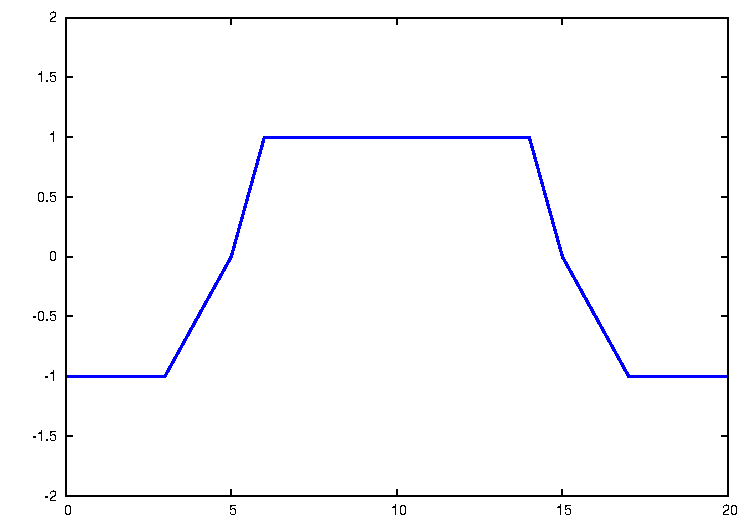
\includegraphics[width=100mm]{figures/kernel}
\caption{Matched filter kernel for a lane width of 10 pixels.}
\label{fig:kernel}
\end{figure}

\subsection{Non-Maximum Suppression}
The results from ``Matched Filter Convolution" consists of the detected lane 
marking and noise. To simplify the processing I used the ``Non-Maximum 
Suppression'' technique to transform a lane marking which has some width to a 
lane marking which which is one pixel wide. The ``Non-Maximum Suppression" used 
here is similar to the one used in edge detectors except that in this case it is 
applied to each row of the image and only take the magnitude of the pixels into 
consideration. 

Figure \ref{fig:non_maxima} shows the effect of applying non-maximum suppression 
to an input signal. 

\begin{figure}
\centering
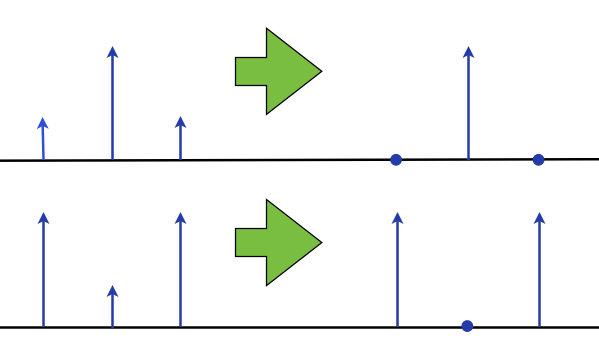
\includegraphics[width=100mm]{figures/non_maxima_suppression.png}
\caption{The effect of applying Non-Maximum Suppression to an input signal.}
\label{fig:non_maxima}
\end{figure}

\section{Connected Component}
After obtaining the results from non-maxima suppression. The pixels that are
close to each other and are likely to belong to the same lane marking needs to
be connected. For this I've used the connected component labeling algorithm 
\fullcite{ConnectedComponent} with slight modification. In the connected 
component algorithm the connectivity is either 4-connected or 8-connected. 

In the 4-connected, connected component labeling algorithm a point $p$ at 
coordinate $(x,y)$ is considered connected if there is another point in it's 4 
neighbors which are:
$$(x+1, y),  (x-1, y), (x, y+1), (x, y-1)$$ 
In the case of the 8-connected the four diagonals neighbors are taken into account as well.
$$(x+1, y+1), (x+1, y-1), (x-1, y+1), (x-1, y-1)$$ 
 
 
\begin{figure}
 \centering
 \begin{tabular}{c c}
   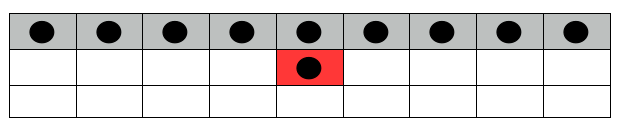
\includegraphics[width=100mm]{figures/connected_component1.png} &
   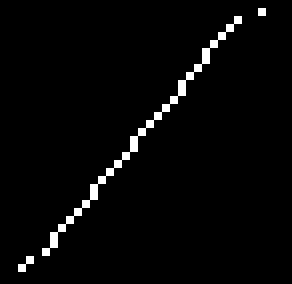
\includegraphics[width=60mm]{figures/pixel_for_connected_component.png} \\
   (a) & (b) \\
 \end{tabular}
 \caption{Connectivity for Connected Component}
 \label{fig:connected_component}
\end{figure}
 
Figure \ref{fig:connected_component}(b) shows a sample of road lane marking that 
needs to be connected. It can be seen that a road lane marking will only have 
one pixel at each row and the closest pixel belonging to the same marking will 
be either on the rows above or below or both. Figure 
\ref{fig:connected_component}(a) shows the connectivity used to connect the 
individual pixels of the road lane marking. The wideness of the connectivity is 
to ensure that all pixel in the lane marking gets connected since the distance 
between any two neighboring pixel in the lane marking varies. 

\section{Image Plane To Ground Plane Transformation}
In order to do further post processing the detected road lanes needs to be 
transformed from the image plane to the ground plane (bird-eye view). 

Equation ~\ref{eq:camera_eq} already describes the relationship between a point in 
the image plane and a point in the real world. Assuming that the ground is flat 
would result in $Z = 0$. Hence equation ~\ref{eq:camera_eq} can be written as: 
\begin{eqnarray*}
\begin{bmatrix}x\\y\\1\end{bmatrix} & = & 
\begin{bmatrix}
p_{11} & p_{12} & p_{13} & p_{14} \\
p_{21} & p_{22} & p_{23} & p_{24} \\
p_{31} & p_{32} & p_{33} & p_{34}
\end{bmatrix}
\begin{bmatrix}X\\Y\\0\\1\end{bmatrix}
\end{eqnarray*}
\begin{eqnarray*}
& = & \begin{bmatrix}
        p_{11} & p_{12} & p_{14} \\
        p_{21} & p_{22} & p_{24} \\
        p_{31} & p_{32} & p_{34}                                            
\end{bmatrix}\begin{bmatrix}X\\Y\\1\end{bmatrix}\\
                                      & = & 
\mathrm{H}\begin{bmatrix}X\\Y\\1\end{bmatrix}
\end{eqnarray*}
Therefore in order to calculate the ground point we can take the inverse of and 
multiply it with the image point. 
\begin{eqnarray*}
\mathrm{H}^{-1} \begin{bmatrix}x\\y\\1\end{bmatrix} & = & 
\begin{bmatrix}X\\Y\\1\end{bmatrix}.
\end{eqnarray*}

\section{Estimating Consistent Lane Marking}

Each lane marking is just a set of points, these points can be represented in 
either the image plane or the ground plane. The transformation was described in 
the previous section. After transforming the lane marking to the ground plane. A 
simple RANSAC line-fitting algorithm is applied to each lane marking this helps 
in removing any outliers that may be present in any lane marking. 

\subsection{Lateral Distance Estimation}
On the roads they are both straight and curved lane marking. 
Sometimes even straight lane marking appear as curved due to the orientation of 
the camera. As of this writing I've assumed all lane marking on to be a line. 

In order to find the lateral distance from the vehicle to each side 
of the lane all the dash lane marking that are consistent must be grouped 
together to form just one line. The following steps describes how consistent 
lane marking are grouped together. 

\begin{enumerate}
\item Randomly select two lane marking.
\item If the two lane marking are not consistent, then repeat step 1.  Two lane marking $L_{1}$ and $L_{2}$ are considered consistent if the following 
conditions are met: 
\[ 
\left(|v_{1} \cdot v_{2}| > \theta_{1} \right) \textbf{ and }
\left(\left|v_{1} \cdot \frac{P_{2} - P_{1}}{\vectornorm{P_{2} - P_{1}}}\right| 
> \theta_{2} \right) \textbf{ and }
\left(\left|v_{2} \cdot \frac{P_{2} - P_{1}}{\vectornorm{P_{2} - P_{1}}}\right| 
> \theta_{3} \right)
\] 
where $v_{1,2}$ are the normalized unit vector representing the line $L_{1,2}$ 
and $p_{1,2}$ is a point that is on the line $L_{1,2}$.
\item Estimate a line $l$ from the two lane marking found in step 2.
\item Using RANSAC find all the lane marking that are consistent with the line 
$l$ formed in the previous step. These consistent lane marking are the inliers 
of line $l$
\item Pick the set that contain the highest amount of inliers.  
\item Remove the inliers found in step 5. 
\item Repeat step 1 until no two lane marking that are consistent with each 
other can be found. 
\end{enumerate}

Once the set of inliers $\mathrm{I} =\{\mathrm{I_{1}}, \mathrm{I_{2}}, . . 
., \mathrm{I_{n}}\}$ where $\mathrm{I_{i}}$ are consistent lane 
marking are found. The distance to the left and right boundary of the lane is 
calculated as follow: 
\begin{enumerate}
  \item Split $\mathrm{I}$ into $\mathrm{I_{L}}$ and $\mathrm{I_{R}}$ where $\mathrm{I_{L}}$ contain inliers which has the closest lane marking on the left side of the origin. Similarly $\mathrm{I_{R}}$ contain inliers which has the closest lane marking on the right side of the origin.
  \item Find the distance from the origin to each inliers in $\mathrm{I_{L}}$ and $\mathrm{I_{R}}$
  \item The  minimum distance to the left and right inliers are assumed to be the distance to the left and right boundary of the lane. 
\end{enumerate}